\documentclass[a4paper,12pt]{article}

\usepackage[utf8]{inputenc}
\usepackage[T1]{fontenc}
\usepackage[spanish]{babel}
\usepackage{amsmath, amssymb}
\usepackage{graphicx}
\usepackage{float}
\usepackage{subcaption}
\usepackage{hyperref}
\usepackage{listings}
\usepackage{xcolor}

% Define colors for syntax highlighting
\definecolor{codegreen}{rgb}{0,0.6,0}
\definecolor{codegray}{rgb}{0.5,0.5,0.5}
\definecolor{codepurple}{rgb}{0.58,0,0.82}
\definecolor{backcolour}{rgb}{0.95,0.95,0.92}

\lstdefinestyle{pythonstyle}{
    language=Python,
    backgroundcolor=\color{backcolour},
    commentstyle=\color{codegreen},
    keywordstyle=\color{magenta},
    numberstyle=\tiny\color{codegray},
    stringstyle=\color{codepurple},
    basicstyle=\ttfamily\footnotesize,
    breakatwhitespace=false,
    breaklines=true,
    captionpos=b,
    keepspaces=true,
    numbers=left,
    numbersep=5pt,
    showspaces=false,
    showstringspaces=false,
    showtabs=false,
    tabsize=4
}
\lstset{style=pythonstyle}



\begin{document}

{\centering \textsf{TFG Pepe}\par}

\vspace{0.5in}

{\huge Martes 3 de marzo de 2026}

\vspace{0.5in}

¡Hola José! No hice todo lo que hablamos la semana pasada, pero pienso que lo que hice da para vernos.

\tableofcontents

\newpage

\section{Sobre la semana pasada}

Implementé el \emph{weight sharing} de los diccionarios de ISTA y el truco para tener más resolución en los mapas de activación. Hice unos experimentos que se pueden ver superficialmente en la siguiente figura y en profundidad en el Anexo.

\begin{figure}[H]
\centering
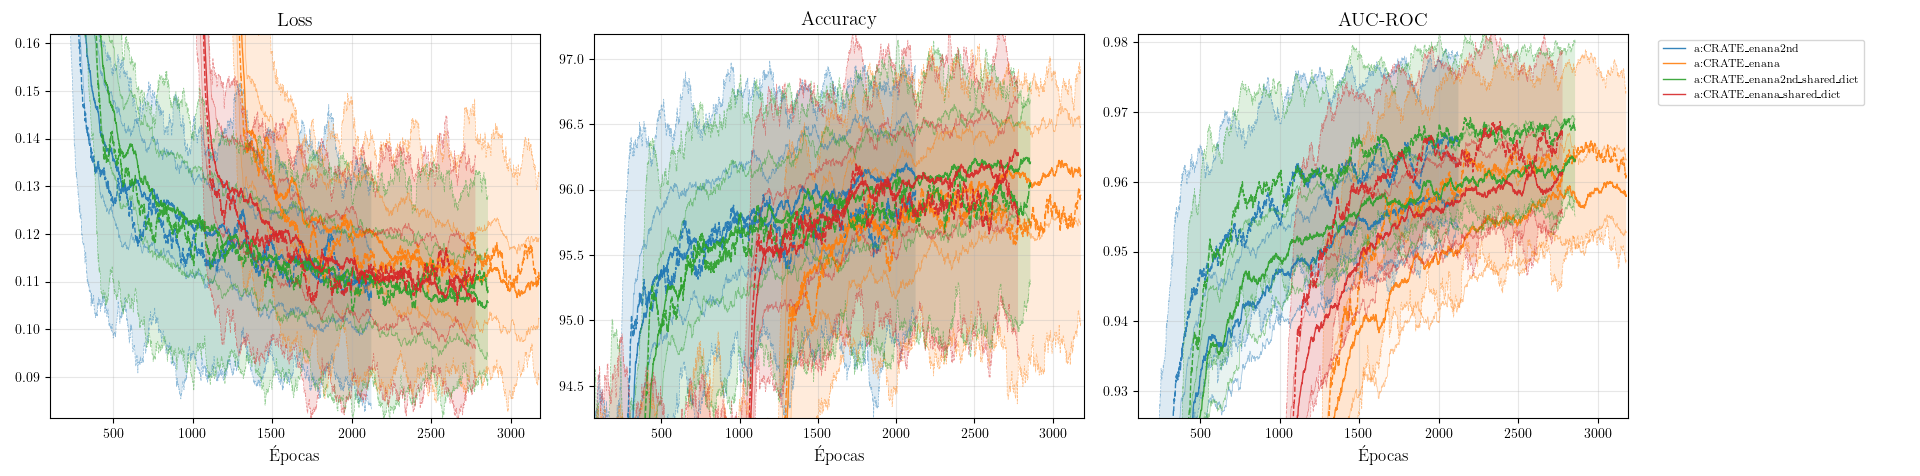
\includegraphics[width=\linewidth]{figs/shared_dict_mediano.png}
\end{figure}

\subsection{\emph{Weight sharing} del diccionario}



Lo cierto es que los entrenamientos son mucho más rápidos, los modelos más pequeños, y los parámetros de los diccionarios en sí más esparsos. También vemos que el Coding Rate mejora en cuanto a que la propiedad de que \emph{las ultimas capas tienen menos CR} (asociada a que la red es un proceso de optimización en si mismo), se acentua levemente.

\subsection{Mapas de activación}

Ahora que son más resolutivos vemos que: las primeras cabezas implementan derivadas primeras de $x$ e $y$ (incluso diría que en la segunda capa se pueden ver resultados estilo filtro LoG) y las atenciones responden a información de ese token y ya, pero en capas más profundas responden a la imagen como un todo (por eso vemos que los tokens de las cabezas finales son más o menos parecidos entre sí, porque la información que portan ya no tiene tanto que ver con el parche de la imagen sino con la tarea (\emph{¿hay vena en el píxel central de la imagen?})). Es por esto que si uno se fija a la forma que tienen las venas cerca del centro, más o menos se puede ver eso en las últimas cabezas, no obstante esto que acabo de decir sólo es cierto para la versión segundo orden, lo cual, en mi opinión le da mérito.

\subsection{Me queda pendiente}

\begin{itemize}
    \item Mezclar órdenes inferencia / entrenamiento.
    \item Desacoplar \emph{positional embeddings}.
\end{itemize}

\section{Configuracion de los experimentos DRIVE}

Te comparto los hiperparametros \emph{comunes} a las distintas ejecuciones; solo por que estén ahí.

\begin{verbatim}
workers: 16
epochs: 5000
label_smoothing: 0.0
batch_size: 4096
lr: 5.0e-05
momentum: 0.9
use_amp: false
weight_decay: 0.001
aumento_datos: true
seed: null
tamano_patch: 75
tamano_token: 15
contador_aumento: -1
overlap_rate: 0.5
label_mode: vainilla
optimizer: AdamW
paciencia: 1000
warmup_steps: 20
class_weight: 1.0
\end{verbatim}

\section{Sobre el coste de la atención}

La semana pasada me recomendaste la lectura de DeepSeek por lo de la mezcla de expertos. Me lo imprimí. Como algo ya conocía de eso por Técnicas Avanzadas del Procesamiento del Lenguaje Natural, y sabía más o menos cómo era el truco, no me motivaba mucho y no me lo leí\ldots\ Busqué y encontré un artículo estupendo: el Linformer \url{https://arxiv.org/pdf/2006.04768}. Su truco es:

\subsection{Linformer}

Imagínate una atención genérica \[ \text{softmax}(Q'K/\sqrt{d})V \] Me venías alertando de la complejidad $\mathcal{O}(n^2)$ porque $Q'$ es $n \times d$; entonces lo que va dentro del softmax es $n \times n$ y luego si multiplicas por $V$ ahí está el tema. Evidentemente tú y yo sabemos de primero de álgebra que lo que va dentro del softmax no puede ser de rango mayor que $d$. Esencialmente el artículo demuestra que la salida del softmax sigue siendo del mismo rango (eso entendí yo). ¿A dónde quiero llegar? Si sabemos que estamos haciendo un producto de matrices grandes de rango bajo, de buena manera podemos hacer un producto de matrices pequeñas de rango completo sin perder información; de forma natural:
\[
    \text{softmax}(Q'KE/\sqrt{d})FV
\]
donde $E$ y $F$ son las matrices de reducción y ampliación de dimensionalidad respectivamente.

\subsection{Revisitando el segundo orden de Neuman}

La semana pasada hablando de esta nueva arquitectura había muchos $ZU$s. Realmente $ZU$ es la pertenencia a las columnas (espacios) de $U$ para cada token.  Por tanto pienso yo que llamarlos $\alpha$ tiene una doble ventaja, ocupa menos tinta y desvela la naturaleza. Si es cierto lo que dice \texttt{DruvPai} y las columnas de U son ortogonales, mi lectura de todo esto esque los vectores $\alpha$ tienen muchos ceros. 

\begin{figure}[H]
\centering
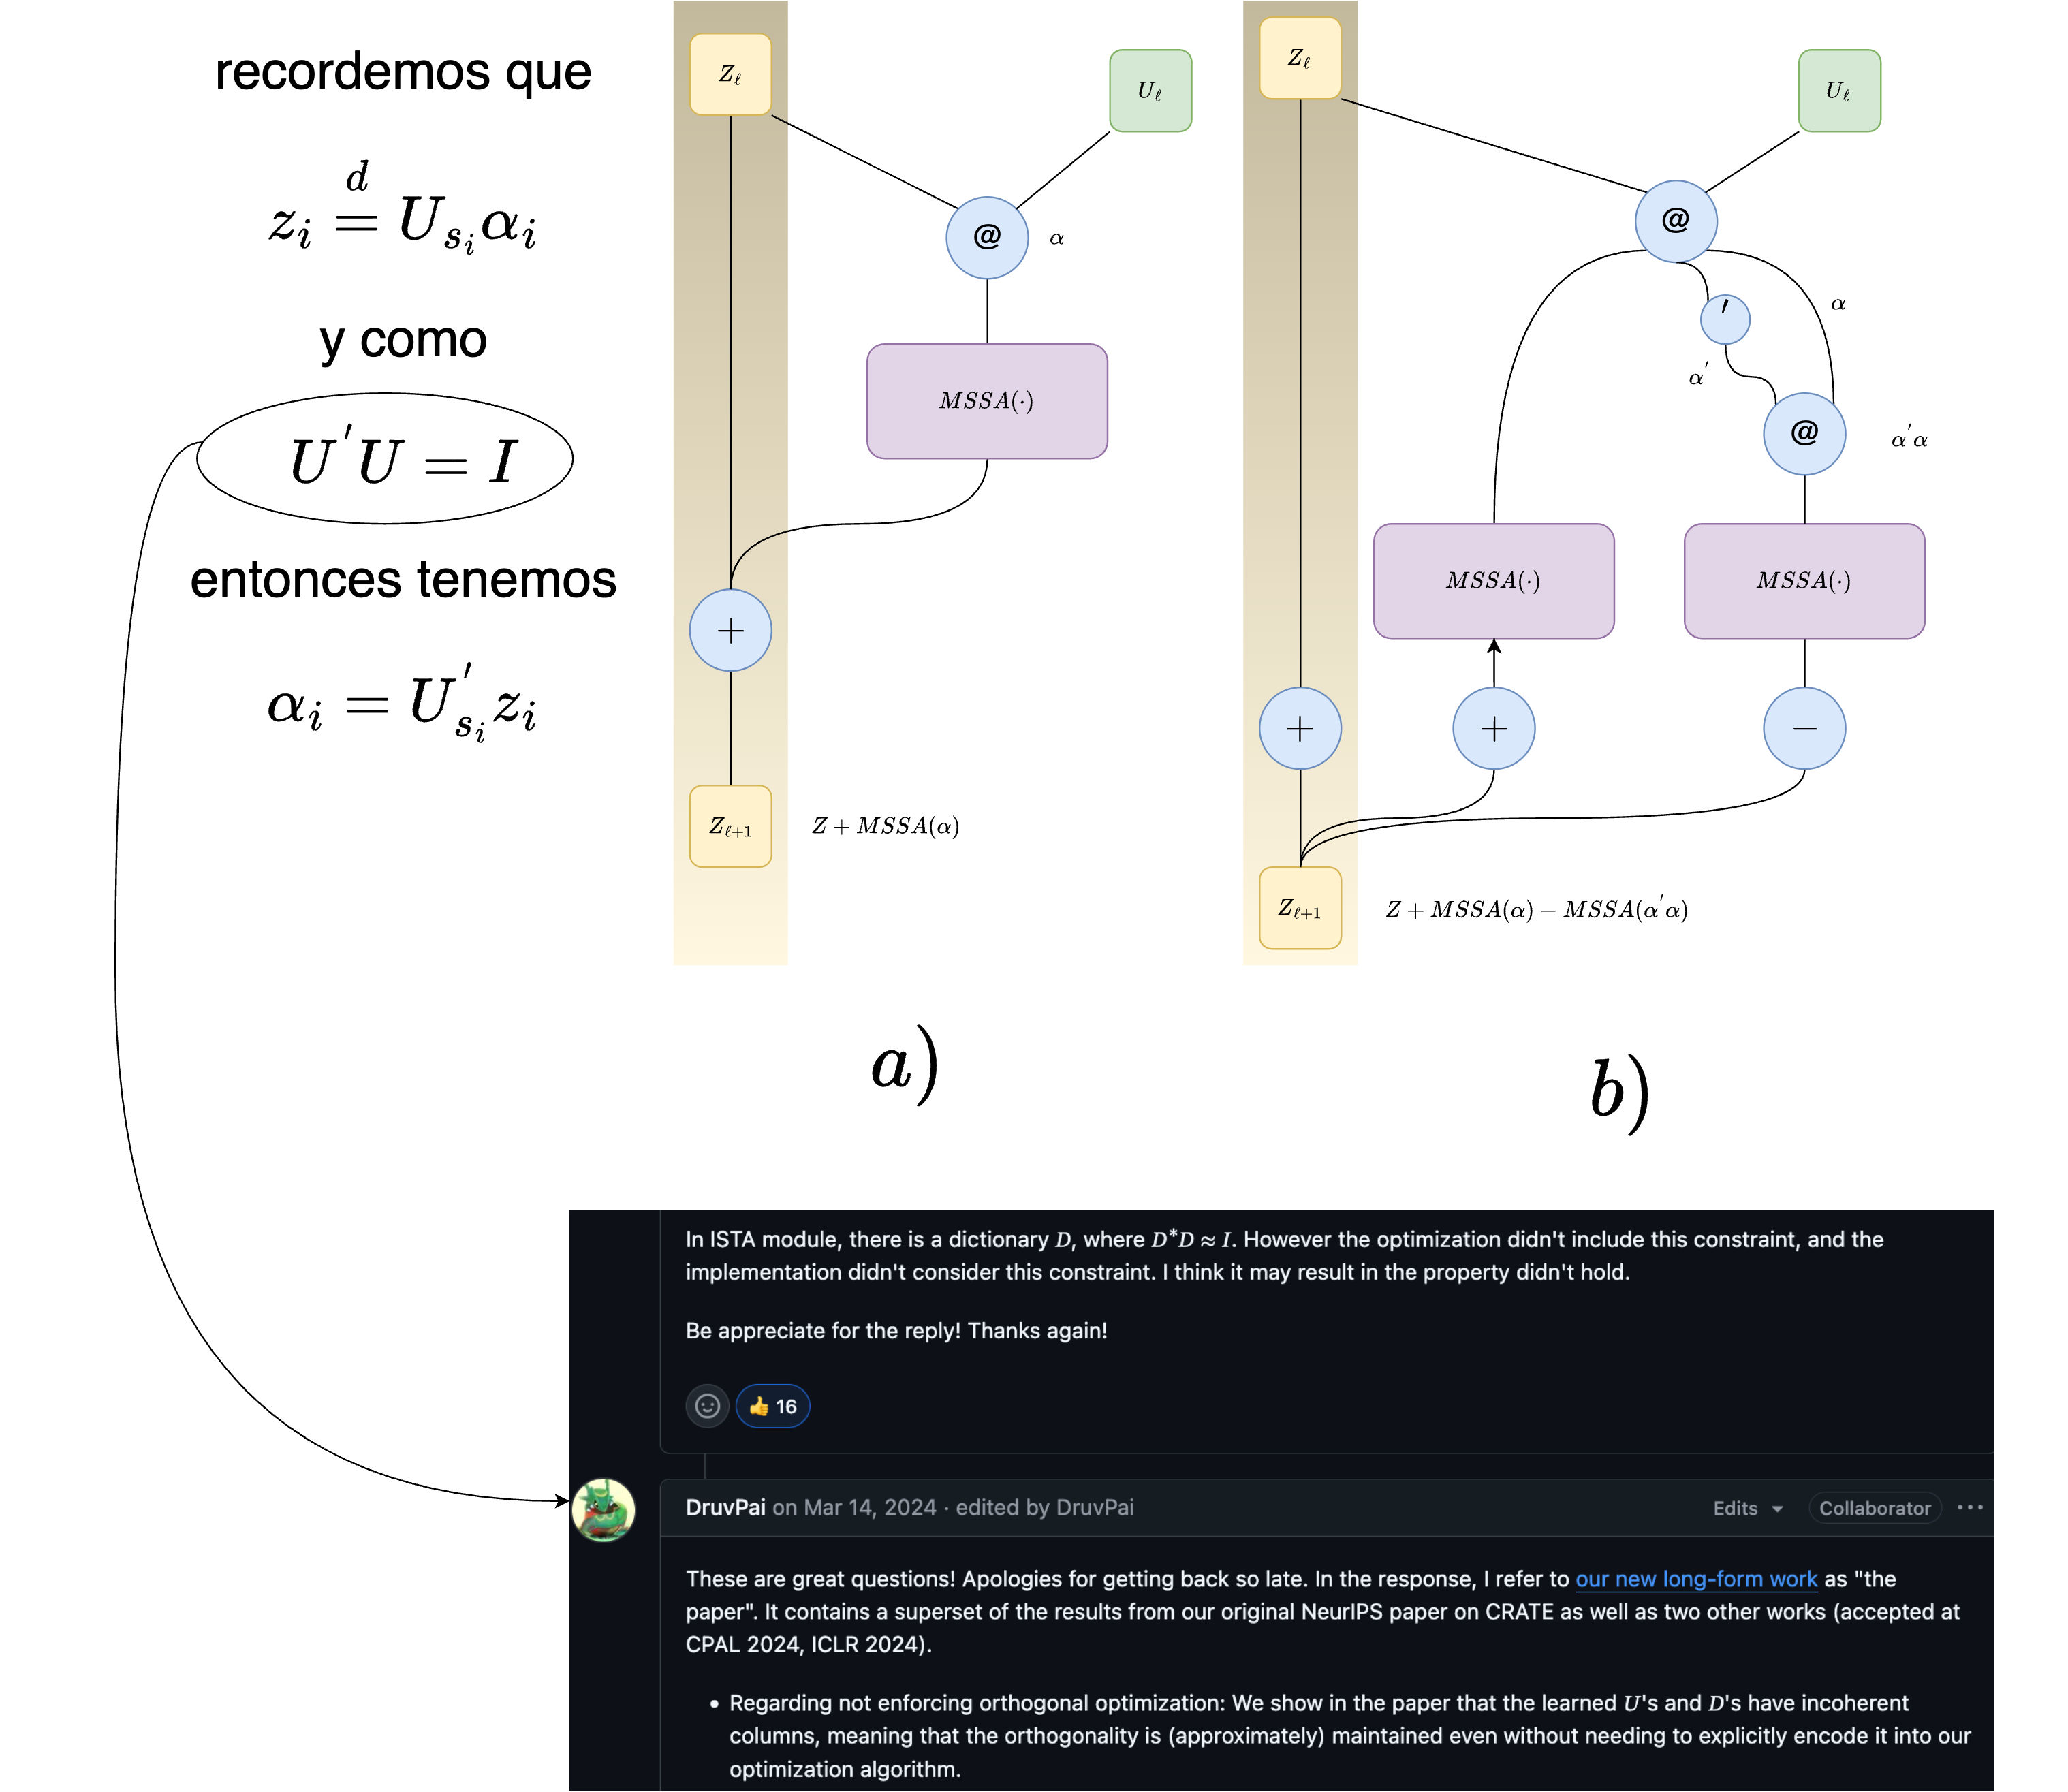
\includegraphics[width=\linewidth]{figs/diagrama_red.drawio.png}
\end{figure}

Hasta aquí no deberia haber nada nuevo (en esta subsección me refiero). Pues bien, tenemos dos cosas: 
\begin{itemize}
	\item Por un lado una nueva arquitectura (la \emph{mía}) que utiliza un \scaps{MSSA} adicional con $\alpha^{'} \alpha$,  como consulta, clave y valor.
	\item Por otro lado una arquitectura, el Linformer, que parte de la premisa de rango pequeño dentro como salida del softmax para acelerar el entrenamiento (y ocupar menos).
\end{itemize}

Sería la ostia que $\alpha^{'} \alpha$ fuese de bajo rango, en ese caso se podría estrujar el Linformer. Implementé en un \texttt{crate.py} (que se convirtió en una factoría) tanto el Linformer como la posibilidad de hacer ambas arquitecturas, pero aún no hice experimentos, porque en DRIVE mis imágenes son de $n = 5 \times 5$ tokens entonces no me parecío apropiado porque me parecía ya suficientemente bajo. Hice muy pequeñas pruebas con RFMiD (leer siguiente sección) y puedo decir que con Linformer puedo tener efectivamente un tamaño de batch mucho más grande.


\section{Necesidad de otra tarea}

Lo cierto es que esta tarea (predecir si el pixel central es vena o no) es muy sencilla. Yo creo que fue apropiada para ir haciendo pruebas y a mí me valió para tener una referencia clara de qué debería hacer el modelo, pero como es una tarea muy simple, no hacen falta ni muchos tokens de entrada ni redes muy grandes, por tanto las cuestiones de rendimiento más o menos se eluden.

Imagina el caso de que implemento el Linformer, y paso de $\mathcal{O}(n^2)$ a $\mathcal{O}(nr)$ donde $r$ es el rango. Pues si $n$ es 5 ó 7 y $r$ es (pongamos) 3 ó 2, hasta seguramente veamos peores rendimientos por el hecho de introducir una matriz más.

Además, pienso que los mapas de activación serán más interesantes porque si pensamos los mapas de activación como el ``razonamiento'' de la red, pues (pienso yo) para una tarea trivial el razonamiento es trivial.


\vspace{0.5in}

Tomé la iniciativa (a expensas de que te parezca mala idea) y fui acomodando el repo a RFMiD\footnote{Lo saqué de  \texttt{https://www.kaggle.com/datasets/andrewmvd/retinal-disease-classification}}, que supongo que ya conoces. No uso la información de que tipo de enfermedad, hago clasificación binaria en enfermo o sano. Más alla de montarlo, poco experimento hice porque RFMiD es más grande el dataset y son más grandes las imágenes; pero lo que hice si me valió para ver que la 


\section{¿Qué creo que tengo que hacer ahora?}

Pues no lo sé, por eso estoy aquí.

\newpage

\section{Extra\ldots}

¡Fui de ayuda a alguien! :D

\begin{figure}[H]
\centering
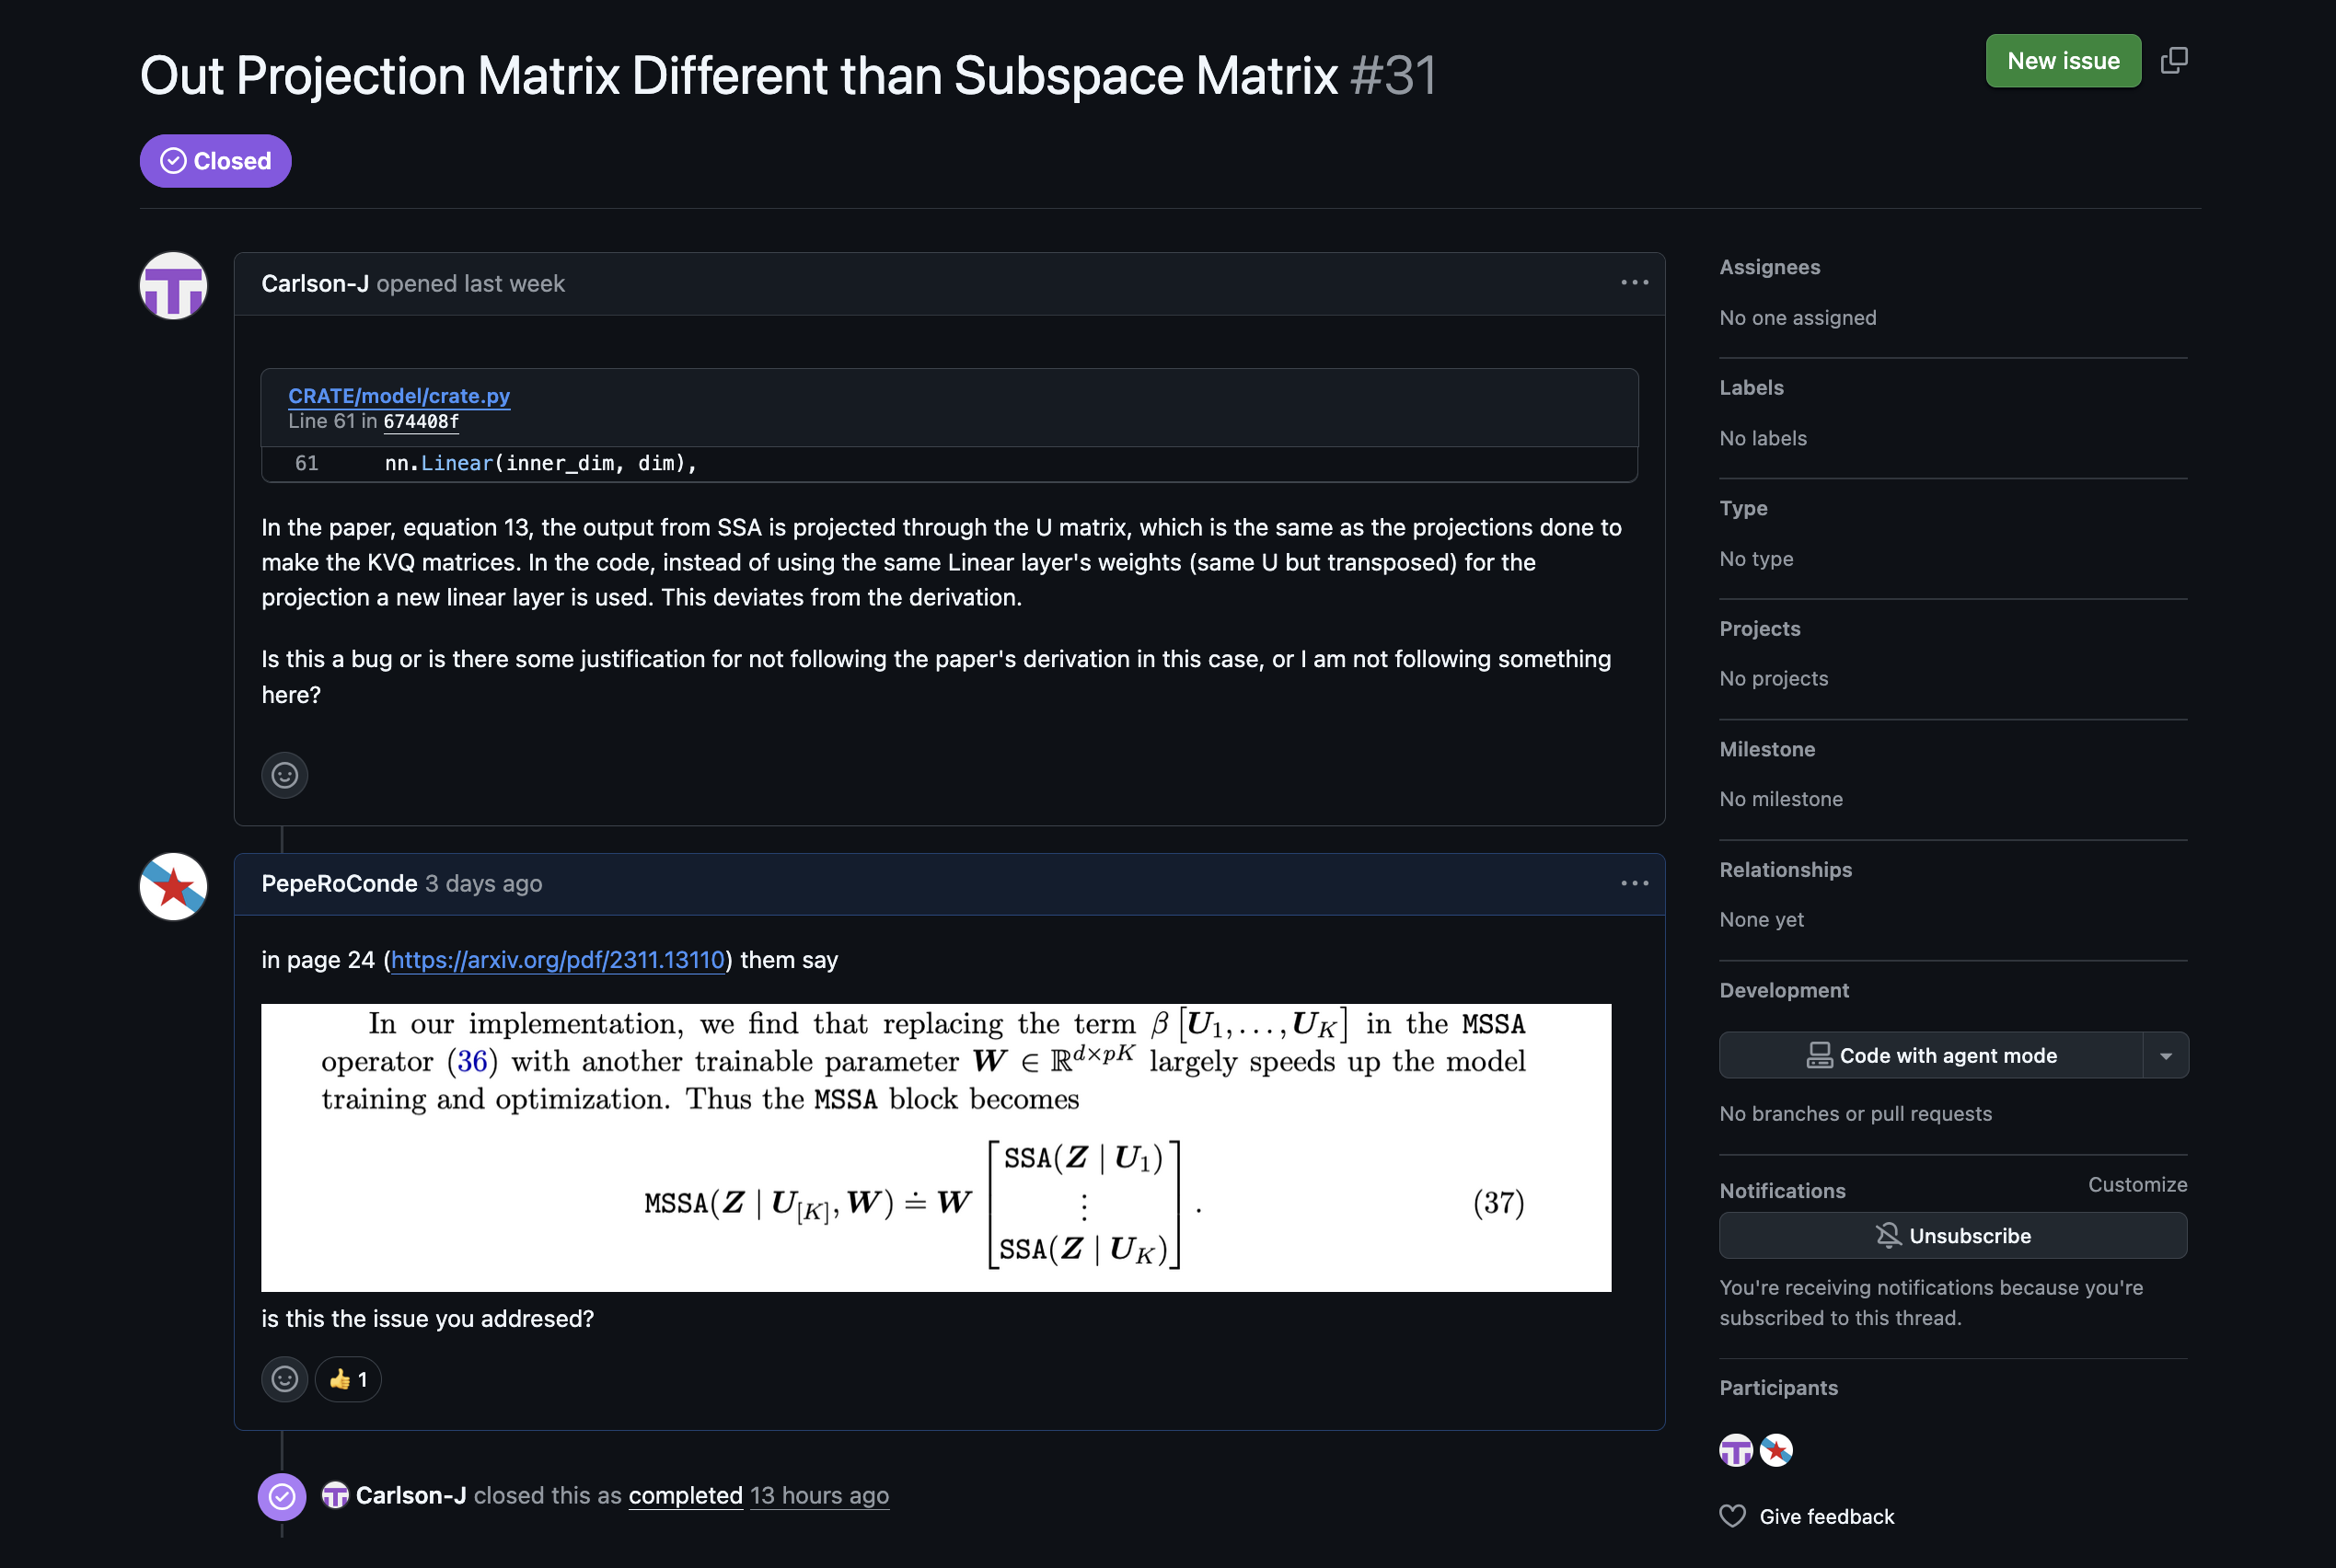
\includegraphics[width=\linewidth]{figs/issue.png}
\end{figure}

\section{Anexo}


% plot de sparsity y tal

\begin{figure}[H]
\centering
\includegraphics[width=\linewidth]{../../data/runs/1vs2_07/plots/03f12c.pth_atencion.png}
\caption{CRATE enana}
\end{figure}

\begin{figure}[H]
\centering
\includegraphics[width=\linewidth]{../../data/runs/1vs2_07/plots/64e36a.pth_atencion.png}
\caption{crate enana, segundo orden}
\end{figure}

\begin{figure}[H]
\centering
\includegraphics[width=\linewidth]{../../data/runs/1vs2_07/plots/994b46.pth_atencion.png}
\caption{CRATE enana, diccionario compartido}
\end{figure}

\begin{figure}[H]
\centering
\includegraphics[width=\linewidth]{../../data/runs/1vs2_07/plots/81e33e.pth_atencion.png}
\caption{CRATE enana, segundo orden, diccionario compartido}
\end{figure}


\begin{figure}[H]
\centering

\begin{subfigure}{0.48\linewidth}
    \centering
    \includegraphics[width=\linewidth]{../../data/runs/1vs2_07/plots/03f12c.pth_complete_inference.png}
    \caption{CRATE enana}
\end{subfigure}
\hfill
\begin{subfigure}{0.48\linewidth}
    \centering
    \includegraphics[width=\linewidth]{../../data/runs/1vs2_07/plots/64e36a.pth_complete_inference.png}
    \caption{CRATE enana, segundo orden}
\end{subfigure}

\vspace{0.5cm}

\begin{subfigure}{0.48\linewidth}
    \centering
    \includegraphics[width=\linewidth]{../../data/runs/1vs2_07/plots/994b46.pth_complete_inference.png}
    \caption{CRATE enana, diccionario compartido}
\end{subfigure}
\hfill
\begin{subfigure}{0.48\linewidth}
    \centering
    \includegraphics[width=\linewidth]{../../data/runs/1vs2_07/plots/81e33e.pth_complete_inference.png}
    \caption{CRATE enana, segundo orden, diccionario compartido}
\end{subfigure}

\caption{No hay mucha diferencia}
\end{figure}

\begin{figure}[H]
\centering

\begin{subfigure}{0.48\linewidth}
    \centering
    \includegraphics[width=\linewidth]{../../data/runs/1vs2_07/plots/03f12c_mcr2.png}
    \caption{CRATE enana}
\end{subfigure}
\hfill
\begin{subfigure}{0.48\linewidth}
    \centering
    \includegraphics[width=\linewidth]{../../data/runs/1vs2_07/plots/64e36a_mcr2.png}
    \caption{CRATE enana, segundo orden}
\end{subfigure}

\vspace{0.5cm}

\begin{subfigure}{0.48\linewidth}
    \centering
    \includegraphics[width=\linewidth]{../../data/runs/1vs2_07/plots/994b46_mcr2.png}
    \caption{CRATE enana, diccionario compartido}
\end{subfigure}
\hfill
\begin{subfigure}{0.48\linewidth}
    \centering
    \includegraphics[width=\linewidth]{../../data/runs/1vs2_07/plots/81e33e_mcr2.png}
    \caption{CRATE enana, segundo orden, diccionario compartido}
\end{subfigure}

\caption{Analisis de Coding rate (menos es mejor). Si bien el segundo orden parece que empeora, compartir diccionario mejora por lo menos la forma, es decir las últimas capas tienen menos (lo cual deseamos y vemos que compartir diccionario contribuye)}
\end{figure}

\begin{figure}[H]
\centering

\begin{subfigure}{0.48\linewidth}
    \centering
    \includegraphics[width=\linewidth]{../../data/runs/1vs2_07/plots/03f12c_sparsity.png}
    \caption{CRATE enana}
\end{subfigure}
\hfill
\begin{subfigure}{0.48\linewidth}
    \centering
    \includegraphics[width=\linewidth]{../../data/runs/1vs2_07/plots/64e36a_sparsity.png}
    \caption{CRATE enana, segundo orden}
\end{subfigure}

\vspace{0.5cm}

\begin{subfigure}{0.48\linewidth}
    \centering
    \includegraphics[width=\linewidth]{../../data/runs/1vs2_07/plots/994b46_sparsity.png}
    \caption{CRATE enana, diccionario compartido}
\end{subfigure}
\hfill
\begin{subfigure}{0.48\linewidth}
    \centering
    \includegraphics[width=\linewidth]{../../data/runs/1vs2_07/plots/81e33e_sparsity.png}
    \caption{CRATE enana, segundo orden, diccionario compartido}
\end{subfigure}

\caption{Analisis de esparsidad. Vemos que compartir diccionario (el diccionario de ISTA) es muy positivo y realmente se nota. El segundo orden en menor medida pero también influye positivamente. ¡Qué bien!}
\end{figure}


\end{document}
